\section{Type Analysis}
\subsection{Types}
\begin{itemize}
	\item The language of type described will be the following possible values
  \begin{align*}
    \tau &\rightarrow \text{int} \\
         & \: | \quad \& \tau \\
         & \: | \quad (\tau, \dots, \tau) \to \tau
  \end{align*}
  \item Which describes the following type terms
  \begin{enumerate}
  	\item Integers
  	\item Heap pointers
  	\item Functions
  \end{enumerate}
  \item Each kind of term has a \textbf{term constructor} that has some arity
  \item For recursive functions and data structures regular types are needed
  \begin{itemize}
    \item They are defined as regular trees using the type constructors
  	\item An infinite tree is regular if it contains only finitely many different subtrees
  \end{itemize}
  \item To describe regular type are the following constructs are part of the language of types 
  \begin{align*}
    \tau &\rightarrow \mu \alpha. \tau \\
         & \: | \quad \alpha \\
         & \: | \quad (\tau, \dots, \tau) \to \tau
  \end{align*}
  \item A type of the form $\mu \alpha . \tau$ is considered identical to the type $\tau[\mu \alpha . \tau / \alpha]$ and is called \textbf{recursive types}
  \item Free type variables are types that are not bound by enclosing $\mu$ and are called \textbf{polymorphic types}
\end{itemize}

\subsection{Type constraints}
\begin{itemize}
	\item For a given program a constraint system is generated
  \begin{itemize}
  	\item A program is defined to be typable when the constraints are solvable 
  \end{itemize}
  \item For type analysis the only constraints considered are equality constraints over regular type terms
  \begin{itemize}
  	\item It can efficiently be solved using a unification algorithm
  \end{itemize}
  \item For each program variable, function parameter and function name $X$ a type variable $\co{X}$ is introduced
  \item For each occurrence of a non-identifier expression $E$ a type variable $\co{E}$ is defined
  \begin{itemize}
  	\item $E$ refers to a concrete node in the abstract syntax i.e. the concrete syntax
  \end{itemize}
  \item The type constraints for TIP:
  \begin{align*} 
    I: & \quad  \co{I} = \text{int} \\
    E_1 \text{ op } E_2: & \quad \co{E_1} = \co{E_2} = \co{E_1 \text{ op } E_2} = \text{int}\\ 
    E_1 == E_2: & \quad \co{E_1} = \co{E_2} \land \co{E_1 == E_2} = \text{int}\\ 
    \text{input}: & \quad \co{\text{input}} = \text{int} \\
    X = E : & \quad \co{X} = \co{E} \\
    \text{output } E : & \quad \co{E} = \text{int} \\
    \text{if } (E) \ S: & \quad \co{E} = \text{int} \\
    \text{if } (E) \ S_1 \text{ else } S_2: & \quad \co{E} = \text{int} \\
    \text{while } (E) \ S: & \quad \co{E} = \text{int} \\
    X(X_1, \dots, X_n)\{\dots \text{return } E;\} : & \quad \co{X} = (\co{X_1}, \dots, \co{X_n}) \rightarrow \co{E} \\
    E(E_1, \dots, E_n) : & \quad \co{E} = (\co{E_1}, \dots, \co{E_n}) \to \co{E(E_1, \dots, E_n)} \\
    \text{alloc } E : & \quad \co{\text{alloc } E} =  \& \co{E} \\
    \& X : & \quad \co{\& X} = \& \co{X} \\
    \text{null} : & \quad \co{\text{null}} = \& \alpha \\
    *E : & \quad \co{E} = \&\co{*E} \\
    *X = E : & \quad \co{X}= \& \co{E}
  \end{align*}
  \item For a complete program constraints are also added to ensure that the parameters and the return value of the \texttt{main} function are \texttt{int}
  \item All term constructors must satisfy the general term equality axiom
  \begin{equation*}
    c(t_1, \dots, t_n) = c'(t_1', \dots, t_n') \Rightarrow t_i = t_i' \text{ for each } i
  \end{equation*}
  \item A \textbf{solution} assign a type to each type variable, such that all equality constraint are satisfied
  \begin{itemize}
  	\item The \textbf{correctness claim} for the type analysis is that the existence of a solution implies that the specified runtime error cannot occur during execution
  \end{itemize}
\end{itemize}

\subsection{Unification solver}
\subsubsection{Union find data structure}
\begin{itemize}
  \item The unification solver uses the union find data structure for representing and manipulating equivalence relations
  \begin{itemize}
  	\item It consist of a direct graph of nodes that have one edge to its parent node
    \item Two nodes are equivalent if they have a common ancestor
  	\item Each root is the canonical representative of its equivalence class
  \end{itemize}
  \item The union find data structure have the following operations:
  \begin{itemize}
    \item $\text{MakeSet}(X)$: adds a new node $x$ that is initially its own parent
    \item $\text{Find}(X$): finds the canonical representative of $x$ by traversing the path to the root, performing path compression on the way
    \begin{itemize}
      \item The parent of each node on the traversed path is set to the canonical representative
    \end{itemize}
    \item $\text{Union}(x,y)$: finds the canonical representative of $x$ and $y$ and makes one parent of the other unless they are already equivalent 
    \end{itemize}
    \item Union find psuedo code:
\begin{lstlisting}[language = pseudocode]
  procedure *@{\sc MakeSet}$(x)$@*
    *@$x.\text{parent} := x$@*
  end procedure

  procedure *@{\sc Find}$(x)$@*
    if*@$x.\text{parent} \neq x$ @*then
      *@$x.\text{parent} := $ {\sc Find}($x.\text{parent}$)@*
    end if
    return*@ $x.\text{parent}$@*
  end procedure

  procedure *@{\sc Union}$(x,y)$@*
    *@$x^r :=$ {\sc Find}$(x)$@*
    *@$y^r :=$ {\sc Find}$(y)$@*
    if *@$x.\text{parent} := y^r$@* then
      *@$x.\text{parent} := y^r$@*
    end if 
  end procedure
\end{lstlisting}
\end{itemize}

\subsubsection{Unification algorithm}
\begin{itemize}
	\item The unification solver can be used to compute solutions to equality constraints
  \item The unification solver only needs to process each constraint once
  \begin{itemize}
  	\item One might interleave generating the constraint and then solving them
  \end{itemize}
  \item The unification algorithm uses union-find by associating a node with each term (including sub-terms) in the constraint system
  \begin{itemize}
	  \item For each term $\tau$ $\text{MakeSet}(\tau)$ is initially invoked
  	\item For each constraint $\tau_1 = \tau_2$ the function $\text{Unify}(\tau_1, \tau_2)$ is invoked which
    \begin{itemize}
      \item unifies the two terms if possible
	    \item enforces the general term equality axiom by unifying sub-terms recursively:
    \end{itemize}
  \end{itemize}
  \item Unification algorithm psudo code
\begin{lstlisting}[language = pseudocode, breaklines=true]
  procedure *@{\sc Unify}$(\tau_1, \tau_2)$@*
    *@$\tau_1^r := $ {\sc Find}($\tau_1$)@*
    *@$\tau_2^r := $ {\sc Find}($\tau_2$)@*
    if *@$\tau_1^r \neq \tau_2^r$@* then
      if *@$\tau_1^r$@* and *@$\tau_2^r$@* are both type variables then
        *@{\sc Union}$(\tau_1^r, \tau_2^r)$@*
      else if *@$\tau_1^r$@* is a type variable and *@$\tau_2^r$@* is a proper type then
        *@{\sc Union}$(\tau_1^r, \tau_2^r)$@*
      else if *@$\tau_1^r$@* is proper type and *@$\tau_2^r$@* is a type variable then 
        *@{\sc Union}$(\tau_2^r, \tau_1^r)$@*
      else if *@$\tau_1^r$@* and *@$\tau_2^r$@* are proper types with the same type constructor then
        *@{\sc Union}$(\tau_1^r, \tau_2^r)$@*
        for each pair of subterms *@$\tau_1'$@* and *@$\tau_2'$@*
          *@{\sc Unify}$(\tau_1', \tau_2')$@*
        end for
      else
        *@\textit{unification failure}@*
      end if
    end if
  end procedure
\end{lstlisting}
\end{itemize}

\subsection{Limitations}
\begin{itemize}
  \item The type analysis is only approximate and therefore certain programs will be unfairly rejected
	\item It is flow-insensitive
	\item It allows dereference of null pointers
	\item It allows escaping stack cell
\end{itemize}

\subsection{Record types}
\begin{itemize}
  \item To extend the type analysis to also work for programs using records, the type language is extended with record types
  \begin{equation*}
    \tau \rightarrow\{X: \tau, \ldots, X: \tau\}
  \end{equation*}
  \item The goal in the analysis is to check that field lookups are only performed on records, not other types of values
	\item A first attempts is to express the type constraints for record construction and field lookup as follows
  \begin{equation*}
    \begin{aligned}
      \left\{X_{1}: E_{1}, \ldots, X_{n}: E_{n}\right\}: & \quad \co{\{X_{1}: E_{1}, \ldots, X_{n}: E_{n}\}}= \{X_1: \co{E_1}, \dots, X_n : \co{E_n}\} \\
      E.X: & \quad \co{E} = \{\dots, X: \co{E.X}, \dots \}
    \end{aligned}
  \end{equation*}
  \item The RHS of the constraint rule for the field lookup is not directly expressible in the language of types
	\item A way to fix this is to require that every record type containts all record fields that exist in the program
  \begin{itemize}
	  \item Let $F = \{f_1,f_2, \dots, f_m\}$ be the set of all field names
	  \item The following two constraint rules is used instead of the previous ones
  \end{itemize}
  \begin{figure}[H]
  	\centering
  	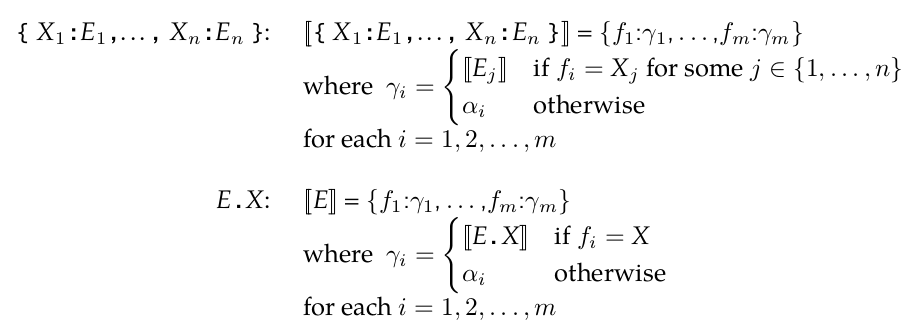
\includegraphics[width=400pt]{img/record_ty}
  \end{figure}
\end{itemize}

\newpage
%%% Local Variables:
%%% mode: latex
%%% TeX-master: "pav-noter"
%%% End:
